% SECTION: Principal Component Analysis (PCA)
\section{Principal Component Analysis (PCA)}

\divider

% SUBSECTION: Problemstellung
\subsection{Problemstellung}

% Problemstellung
\begin{frame}{Problemstellung}{}
	\begin{itemize}
		\item Die \keyword{Principal Component Analysis (PCA)} projiziert hochdimensionale Daten \textit{orthogonal} 
			auf einen \textit{linearen Raum} niederer Dimension.
		\item Diesen linearen Raum nennt man auch \keyword{Principal Subspace}.
		\item Wir betrachten im Folgenden einen Datensatz $\{ \bx_n \}$ mit $n = 1, 2, \ldots, N$ und $\bx_n \in \R^M$.
		\item Unser Ziel ist die Projektion der Daten in einem Raum der Dimension $D$, wobei $D \ll M$.
		\item Für die PCA gibt es verschiedene Ansätze, die zu demselben Ergebnis führen.
		\item Die bekanntesten sind die \keyword{Maximum Variance} Formulierung und die
			\keyword{Minimum Error} Formulierung.
		\item Zunächst wiederholen wir, was man unter der orthogonalen Projektion von Vektoren versteht.
	\end{itemize}
\end{frame}


% SUBSECTION: Orthogonale Projektionen
\subsection{Orthogonale Projektionen}

% Visualisierung: Orthogonale Projektionen
\begin{frame}{Visualisierung: Orthogonale Projektionen}{}
	\begin{figure}
		\centering
		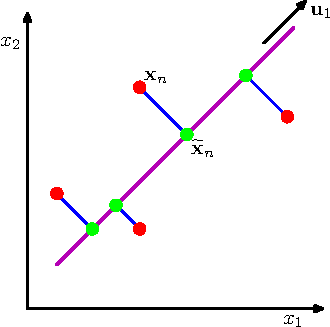
\includegraphics[scale=0.85]{./img/pca/orthogonal_projection}
		\caption{Orthogonale Projektion der Daten $\{ \bx_n \}$ auf die von $\bu_1$ definierte Gerade.
			Siehe \cite{Bishop2024}, Seite 467.}
	\end{figure}
\end{frame}


% Geometrisches Skalarprodukt
\begin{frame}{Geometrisches Skalarprodukt}{}
	\begin{mytheo}[th:pca-geom-scalar-product]
		Es seien $\ba, \bb \in \R^M$. Es gilt das geometrische Skalarprodukt
		$\ba^\top \bb = \Vert \ba \Vert \cdot \Vert \bb \Vert \cdot \cos \angle(\ba, \bb)$.
	\end{mytheo}

	\begin{myproof}
		Für $\Vert \ba - \bb \Vert^2 = (\ba - \bb)^\top (\ba - \bb)$ ergibt sich durch Ausmultiplizieren zum Einen
		\begin{equation} \label{eq:pca-geom-scalar-product-1}
			\begin{aligned}
				\Vert \ba - \bb \Vert^2
					&= \ba^\top \ba - \ba^\top \bb - \bb^\top \ba + \bb^\top \bb
			\\[2mm]
					&= \Vert \ba \Vert^2 + \Vert \bb \Vert^2 - 2 \ba^\top \bb
			\end{aligned}
		\end{equation}
		und zum Anderen aufgrund des \keyword{Kosinussatzes} (Verallgemeinerung des Satzes von Pythagoras)
		aus der Geometrie
		\begin{equation} \label{eq:pca-geom-scalar-product-2}
			\Vert \ba - \bb \Vert^2
				= \Vert \ba \Vert^2 + \Vert \bb \Vert^2
				- 2 \cdot \Vert \ba \Vert \cdot \Vert \bb \Vert \cdot \cos \angle(\ba, \bb).
		\end{equation}
		Setzt man die Ausdrücke \eqref{eq:pca-geom-scalar-product-1} und \eqref{eq:pca-geom-scalar-product-2} für
		$\Vert \ba - \bb \Vert^2$ gleich, subtrahiert auf beiden Seiten $\Vert \ba \Vert^2 + \Vert \bb \Vert^2$ und
		dividiert durch $-2$, so ergibt sich $\ba^\top \bb = \Vert \ba \Vert \cdot \Vert \bb \Vert \cdot \cos \angle(\ba, \bb)$,
		die Behauptung.
	\end{myproof}
\end{frame}


% Orthogonalität von Vektoren
\begin{frame}{Orthogonalität von Vektoren}{}
	\begin{mytheo}[th:pca-orth-vector-scalar-prod]
		Es seien $\ba, \bb \in \R^M$ verschieden von $\0$. Es gilt $\ba^\top \bb = 0$ genau dann,
		wenn $\ba$ und $\bb$ orthogonal aufeinander stehen.
	\end{mytheo}

	\begin{myproof}
		Wenn die Vektoren $\ba$ und $\bb$ orthogonal, d.\,h. senkrecht, aufeinander stehen, dann gilt
		$\cos \angle(\ba, \bb) = 0$, da die Kosinus-Funktion bei $\pi/2$ (entspricht 90°) eine Nullstelle hat.
		Mit Satz \ref{th:pca-geom-scalar-product} folgt
		\begin{equation*}
			\ba^\top \bb
				= \Vert \ba \Vert^2 \cdot \Vert \bb \Vert^2 \cdot \cos \angle(\ba, \bb)
				= \Vert \ba \Vert^2 \cdot \Vert \bb \Vert^2 \cdot 0
				= 0.
		\end{equation*}
		Sei nun $\ba^\top \bb = 0$. Da die Vektoren von $\0$ verschieden sind, muss wegen der Eigenschaften der Norm
		zwingend $\cos \angle(\ba, \bb) = 0$ gelten. Die Vektoren stehen also senkrecht aufeinander. Damit gilt die Behauptung.
	\end{myproof}
\end{frame}


% Orthogonale Projektion von Vektoren
\begin{frame}{Orthogonale Projektion von Vektoren}{}
	\begin{mytheo}[th:pca-orth-proj]
		Es seien $\ba, \bb \in \R^M$. Dann ist die orthogonale Projektion von $\bb$ auf $\ba$ gegeben durch
		\begin{equation*}
			\proj_{\ba} \bb = \frac{\ba^\top \bb}{\Vert \ba \Vert^2} \ba.
		\end{equation*}
	\end{mytheo}

	\begin{myproof}
		Es müssen zwei Bedingungen erfüllt sein. Einerseits ist der Projektionsvektor
		$\bp \coloneqq \proj_{\ba} \bb$ der Anteil von $\bb$,
		der in Richtung $\ba$ zeigt, sodass dieser eine Stauchung bzw. Streckung von $\ba$ ist. Mit $k \in \R$ gilt also
		\begin{equation} \label{eq:pca-orth-proj-1}
			\bp = k \cdot \ba.
		\end{equation}
		Andererseits soll die Projektion orthogonal sein, d.\,h. wir wollen den Vektor $\bp$ so finden,
		dass $\bb - \bp$ senkrecht auf $\ba$ steht. Mit Satz \ref{th:pca-orth-vector-scalar-prod} lautet die Bedingung also
		\begin{equation} \label{eq:pca-orth-proj-2}
			(\bb - \bp)^\top \ba = 0.
		\end{equation}
		Einsetzen von \eqref{eq:pca-orth-proj-1} in \eqref{eq:pca-orth-proj-2} und auflösen nach $k$ ergibt
		$(\bb - k \cdot \ba)^\top \ba = 0 \Longleftrightarrow k = \frac{\ba^\top \bb}{\Vert \ba \Vert^2}$.
		Dieses Ergebnis setzen wir in \eqref{eq:pca-orth-proj-1} ein und erhalten die Behauptung.
	\end{myproof}
\end{frame}


% Orthogonale Projektion von Vektoren (Forts.)
\begin{frame}{Orthogonale Projektion von Vektoren (Forts.)}{}
	\begin{figure}
		\begin{tikzpicture}[
	scale=0.8
]
	\coordinate (A) at ($(0,0)!(3,4)!(5,1)$);
	\draw[dashed,thick] (3,4) -- (A);
		
	\draw[ultra thick,red,-stealth] (0,0) -- (5,1) node[right] {$\ba$};
	\draw[very thick,purple,-stealth] (0,0) -- (A) node[below=2mm] {$\proj_{\ba} \bb$};
	\draw[very thick,blue,-stealth] (0,0) -- (3,4) node[right] {$\bb$};
\end{tikzpicture}

		\caption{Projektion des Vektors $\bb \in \R^2$ auf den Vektor $\ba \in \R^2$.
		Im Kontext der PCA ist der Vektor $\ba$ der Principal Subspace $\bu_1$ und $\bb$ ist ein Datenpunkt,
		der auf diesen Raum projiziert wird.}
	\end{figure}
\end{frame}


% Orthogonale Projektion von Vektoren (Forts.)
\begin{frame}{Orthogonale Projektion von Vektoren (Forts.)}{}
	\begin{itemize}
		\item Interessieren wir uns nur für die \textit{Länge des Projektionsvektors}, so betrachten wir seine Norm
		\begin{equation}
			\Vert \proj_{\ba} \bb \Vert
				= \frac{\ba^\top \bb}{\Vert \ba \Vert^2} \Vert \ba \Vert
				= \frac{\ba^\top \bb}{\Vert \ba \Vert}.
		\end{equation}
		\item Gilt zudem $\Vert \ba \Vert = 1$ (dann ist $\ba$ ein Einheitsvektor),
			so ergibt sich die Länge des Projektionsvektors einfach als das Skalarprodukt der beteiligten Vektoren
		\begin{equation}
			\Vert \proj_{\ba} \bb \Vert = \ba^\top \bb.
		\end{equation}
		\item Wir gehen im Folgenden davon aus, dass die \keyword{Principal Components} $\{ \bu_i \}$ normiert sind.
	\end{itemize}
\end{frame}


% SUBSECTION: Maximum-Variance Formulierung der PCA
\subsection{Maximum-Variance Formulierung der PCA}

% Maximum-Variance Formulierung
\begin{frame}{Maximum-Variance Formulierung}{}
	\begin{itemize}
		\item Im Folgenden betrachten wir den Fall $D = 1$.
		\item Wir betrachten also nur eine einzelne Principal Component $\bu_1$.
		\item Eine mögliche Formulierung der PCA ist es, die \textit{Varianz der projizierten Daten zu maximieren}.
		\item Durch die Maximierung der Varianz erhofft man sich den Erhalt eines möglichst großen Anteils
			der Struktur der Daten.
		\item Dieses Vorgehen führt auf die \keyword{Maximum-Variance Formulierung} der PCA.
		\item Da $\Vert \bu_1 \Vert = 1$, ist die Projektion eines Datenpunkts $\bx_n$ auf $\bu_1$ gegeben durch
		\begin{equation} \label{eq:pca-projection-data}
			\tilde{x}_n = \bu_1^\top \bx_n.
		\end{equation}
	\end{itemize}

	\begin{boxGray}
		\begin{center}
			\textbf{Ziel:} Finde $\bu_1$ so, dass die Varianz der Projektionen $\{ \tilde{x}_n \}$ maximal wird.
		\end{center}
	\end{boxGray}
\end{frame}


% Projektion von Mittelwert und Varianz
\begin{frame}{Projektion von Mittelwert und Varianz}{}
	\begin{itemize}
		\item Der Mittelwert der projizierten Daten ist analog gegeben durch
		\begin{equation} \label{eq:pca-projection-mean}
			\bu_1^\top \bxmean,
		\qquad\text{mit}\qquad
			\bxmean \coloneqq \frac{1}{N} \sum_{n=1}^N \bx_n.
		\end{equation}
		\item Die projizierte Varianz bestimmt man mittels
		\begin{equation} \label{eq:pca-projection-variance}
			\bu_1^\top \bS \bu_1.
		\end{equation}
		\item Hierbei bezeichnet $\bS$ die \keyword{Streuungsmatrix} der Daten im hochdimensionalen Raum.
		\item Sie ist gegeben durch
		\begin{equation} \label{eq:pca-scatter-matrix}
			\bS \coloneqq \frac{1}{N} \sum_{n=1}^N (\bx_n - \bxmean) (\bx_n - \bxmean)^\top.
		\end{equation}
	\end{itemize}
\end{frame}


% Beweis von \eqref{eq:pca-projection-variance}
\begin{frame}{Beweis von \eqref{eq:pca-projection-variance}}{}
	Wir beweisen Gleichung \eqref{eq:pca-projection-variance}: \\ \vspace*{2mm}
	\begin{myproof}
		Wir setzen die Projektionen \eqref{eq:pca-projection-data} und \eqref{eq:pca-projection-mean} in die Definition
		der Varianz ein und erhalten durch Ausmultiplizieren aufgrund der Symmetrie des Skalarprodukts
		\begin{align*}
			\frac{1}{N} \sum_{n=1}^N \Bigl( \bu_1^\top \bx_n - \bu_1^\top \bxmean \Bigr)^2
				&= \frac{1}{N} \sum_{n=1}^N \Bigl(
					\bu_1^\top \bx_n \cdot \bx_n^\top \bu_1 - 2 \cdot \bu_1^\top \bx_n \cdot \bxmean^\top \bu_1
						+ \bu_1^\top \bxmean \cdot \bxmean^\top \bu_1
				\Bigr)
		\\[2mm]
				&= \bu_1^\top \left(
					\frac{1}{N} \sum_{n=1}^N \Bigl( \bx_n \bx_n^\top - 2 \cdot \bx_n \bxmean^\top + \bxmean\bxmean^\top \Bigr)
				\right) \bu_1
		\\[2mm]
				&= \bu_1^\top \left( \frac{1}{N} \sum_{n=1}^N (\bx_n - \bxmean) (\bx_n - \bxmean)^\top \right) \bu_1
		\\[2mm]
				&= \bu_1^\top \bS \bu_1.
				&& \rem{Einsetzen von \eqref{eq:pca-scatter-matrix}.}
		\end{align*}
	\end{myproof}
\end{frame}


% Maximierung der projizierten Varianz
\begin{frame}{Maximierung der projizierten Varianz}{}
	\begin{itemize}
		\item Unser Ziel ist nun die Maximierung der projizierten Varianz $\bu_1^\top \bS \bu_1$ in $\bu_1$.
		\item \textbf{Problem:} Dieses Maximierungsproblem ist unbeschränkt.
		\item Wir können diesen Ausdruck stets vergrößern, indem wir die Komponenten von $\bu_1$ vergrößern.
		\item Um dies zu verhindern, fordern wir, dass $\Vert \bu_1 \Vert = 1$ gilt.
	\end{itemize}

	\begin{boxGray}
		\textbf{Maximierungsproblem für die PCA:}
		\begin{equation} \label{eq:pca-max-var-problem}
			\begin{aligned}
				\text{Maximiere} 	&\qquad \bu_1 \bS \bu_1
			\\[2mm]
				\text{unter} 		&\qquad \Vert \bu_1 \Vert = 1.
			\end{aligned}
		\end{equation}
	\end{boxGray}
\end{frame}


% Maximierung der projizierten Varianz (Forts.)
\begin{frame}{Maximierung der projizierten Varianz (Forts.)}{}
	\begin{itemize}
		\item Löst man Problem \eqref{eq:pca-max-var-problem}, so erhält man für $\bu_1$ die Bedingung
		\begin{equation} \label{eq:pca-eigenvalue-problem}
			\bS \bu_1 = \lambda_1 \bu_1.
		\end{equation}
		\item Gleichung \eqref{eq:pca-eigenvalue-problem} sagt aus, dass $\bu_1$ ein Eigenvektor von $\bS$ sein muss.
		\item Der Lagrange-Multiplikator $\lambda_1$ ist der zugehörige Eigenwert.
	\end{itemize}

	\begin{mytask}
		Zeigen Sie die Gültigkeit von \eqref{eq:pca-eigenvalue-problem}, indem Sie das
		Optimierungsproblem \eqref{eq:pca-max-var-problem} lösen. Stellen Sie hierzu die Lagrange-Funktion des Problems auf
		und finden Sie deren stationären Punkte.
	\end{mytask}
\end{frame}


% Maximierung der projizierten Varianz (Forts.)
\begin{frame}{Maximierung der projizierten Varianz (Forts.)}{}
	\begin{itemize}
		\item Multiplizieren wir \eqref{eq:pca-eigenvalue-problem} von links mit $\bu_1^\top$, so erhalten wir
		\begin{equation} \label{eq:pca-retained-variance}
			\bu_1^\top \bS \bu_1 = \lambda_1 \bu_1^\top \bu_1 = \lambda_1 \Vert \bu_1 \Vert^2 = \lambda_1.
		\end{equation}
		\item Im letzten Gleichheitszeichen haben wir benutzt, dass eine Lösung von \eqref{eq:pca-max-var-problem}
			die Nebenbedingung $\Vert \bu_1 \Vert = 1$ erfüllt.
		\item Wegen \eqref{eq:pca-retained-variance} ist der Eigenwert $\lambda_1$ die Varianz, die durch Projektion der Daten
			auf $\bu_1$ erhalten bleibt.
	\end{itemize}

	\begin{boxGray}
		\textbf{Lösung für den Fall $D = 1$:} Wir berechnen die Eigenzerlegung von $\bS$ und benutzen als $\bu_1$
		einen (normierten) Eigenvektor zum größten Eigenwert. Wegen \eqref{eq:pca-retained-variance} erhält dieser den
		größten Anteil der Varianz.
	\end{boxGray}
\end{frame}


% Bestimmung weiterer Principal Components
\begin{frame}{Bestimmung weiterer Principal Components}{}
	\begin{itemize}
		\item Die Bestimmung weiterer Principal Components ist einfach.
		\item Wir benutzen als $\bu_2$ einen normierten Eigenvektor von $\bS$ zum zweitgrößten Eigenwert $\lambda_2$.
		\item Wir benutzen als $\bu_3$ einen normierten Eigenvektor von $\bS$ zum drittgrößten Eigenwert $\lambda_3$.
		\item Dies führen wir solange fort, bis wir die vorgegebenen $D$ Komponenten erreicht haben.
		\item Wir fassen die Vektoren $\bu_1, \bu_2, \ldots, \bu_D$ in einer Matrix $\bV \in \R^{M \times D}$ zusammen.
		\item Die Projektionen $\bXtilde \in \R^{N \times D}$ der Daten $\bX \in \R^{N \times M}$ erhalten wir dann mittels
		\begin{equation}
			\bXtilde = \bX \bV.
		\end{equation}
	\end{itemize}
\end{frame}


% Orthogonalität der Principal Components
\begin{frame}{Orthogonalität der Principal Components}{}
	\begin{mytheo}
		Die Principal Components $\{ \bu_i \}$ stehen senkrecht aufeinander.
	\end{mytheo}

	\begin{myproof}
		Dies folgt direkt aus der Orthogonalität der Eigenvektoren von symmetrischen Matrizen zu verschiedenen Eigenwerten.
		Seien also $\lambda_1$ und $\lambda_2$ mit $\lambda_1 \ne \lambda_2$ zwei voneinander verschiedene Eigenwerte
		von $\bS$. Dann erfüllen diese die Gleichungen $\bS \bu_1 = \lambda_1 \bu_1$ und $\bS \bu_2 = \lambda_2 \bu_2$.
		Damit gilt
		\begin{equation} \label{eq:pca-princ-comp-orth-1}
			\bigl( \bS \bu_1 \bigr)^\top \bu_2
				= \bigl( \lambda_1 \bu_1 \bigr)^\top \bu_2
				= \lambda_1 \bu_1^\top \bu_2.
		\end{equation}
		Außerdem gilt aufgrund der Symmetrie von $\bS$ und der Tatsache, dass man eine Matrix im Skalarprodukt
		transponiert auf die andere Seite bringen darf
		\begin{equation} \label{eq:pca-princ-comp-orth-2}
			\bigl( \bS \bu_1 \bigr)^\top \bu_2
				= \bu_1^\top \bigl( \bS^\top \bu_2 \bigr)
				= \bu_1^\top \bigl( \bS \bu_2 \bigr).
		\end{equation}
		Nun setzen wir die Eigenwertgleichung in \eqref{eq:pca-princ-comp-orth-2} ein und erhalten
		\begin{equation} \label{eq:pca-princ-comp-orth-3}
			\bigl( \bS \bu_1 \bigr)^\top \bu_2
				= \bu_1^\top \bigl( \lambda_2 \bu_2 \bigr)
				= \lambda_2 \bu_1^\top \bu_2.
		\end{equation}
		Setzt man nun \eqref{eq:pca-princ-comp-orth-1} und \eqref{eq:pca-princ-comp-orth-2} gleich, so erhält man
		schlussendlich $(\lambda_1 - \lambda_2) \cdot \bu_1^\top \bu_2 = 0$. Da $\lambda_1 \ne \lambda_2$ muss
		$\bu_1^\top \bu_2 = 0$ gelten. Mit Satz \ref{th:pca-orth-vector-scalar-prod} folgt die Behauptung.
	\end{myproof}
\end{frame}


% SUBSECTION: PCA-Algorithmus
\subsection{PCA-Algorithmus}

% PCA-Algorithmus
\begin{frame}{PCA-Algorithmus}{}
	\begin{myalg}
		\begin{enumerate}
			\item Bestimme $\bxmean$ und $\bS$ gemäß \eqref{eq:pca-projection-mean} beziehungsweise
				\eqref{eq:pca-scatter-matrix}.
			\item Berechne die Eigenzerlegung von $\bS$, d.\,h. finde Matrizen $\bU$ und $\bLambda$ mit
				$$\bS = \bU \bLambda \bU^\top.$$ Dabei enthält die Matrix $\bU \in \R^{M \times M}$ die
				Eigenvektoren von $\bS$. $\bLambda \in \R^{M \times M}$ ist eine Diagonalmatrix
				mit den Eigenwerten auf der Hauptdiagonalen.
			\item Normiere die Eigenvektoren, die zu den $D$ größten Eigenwerten gehören und fasse sie in der Matrix
				$\bV \in \R^{M \times D}$ zusammen.
			\item Berechne die Projektionen $\bXtilde = \bX \bV$.
		\end{enumerate}
	\end{myalg}
\end{frame}


% PCA-Algorithmus (Forts.)
\begin{frame}{PCA-Algorithmus (Forts.)}{}
	\begin{mytask}
		Es sei der zweidimensionale Datensatz
		\begin{equation*}
			\bX \coloneqq \begin{pmatrix} 1 & 4 \\ 4 & 1 \\ 1 & 1 \end{pmatrix} \in \R^{3 \times 2}
		\end{equation*} gegeben. Berechnen Sie die eindimensionalen Projektionen dieses Datensatzes
		mit dem PCA-Algorithmus.
	\end{mytask}
\end{frame}


% SUBSECTION: Minimum-Error Formulierung der PCA
\subsection{Minimum-Error Formulierung der PCA}

% Minimum-Error Formulierung
\begin{frame}{Minimum-Error Formulierung}{}
	\begin{itemize}
		\item Wir betrachten im Folgenden eine weitere Formulierung der PCA, welche auf der \textit{Minimierung des Projektionsfehlers} basiert,
			die \keyword{Minimum-Error} Formulierung.
		\item Dazu seien $\{ \bu_i \}$ mit $i = 1, 2, \ldots, M$ \textit{orthonormale Basisvektoren}, d.\,h.
		\begin{equation} \label{eq:pca-orthonormality}
			\bu_i^\top \bu_j = \delta_{ij} \qquad \forall\,i, j.
		\end{equation}
		\item Die Basis $\{ \bu_i \}$ ist \textit{vollständig}, weshalb sich jedes $\bx_n$ \textit{eindeutig} als Linearkombination der $\bu_i$ darstellen lässt
		\begin{equation} \label{eq:pca-linear-combination}
			\bx_n = \sum_{i=1}^M \alpha_{ni} \bu_i.
		\end{equation}
		\item Dies entspricht einer Drehung des Koordinatensystems.
	\end{itemize}
\end{frame}


% Minimum-Error Formulierung (Forts.)
\begin{frame}{Minimum-Error Formulierung (Forts.)}{}
	\begin{itemize}
		\item Die Koeffizienten $\alpha_{nj}$ ergeben sich als Projektionen der $\bx_n$ auf die $\bu_j$.
		\item Wegen \eqref{eq:pca-orthonormality} ist $\alpha_{nj} = \bx_n^\top \bu_j$, sodass wir \eqref{eq:pca-linear-combination} schreiben
			können als
		\begin{equation} \label{eq:pca-linear-combination-2}
			\bx_n = \sum_{i=1}^M \bigl( \bx_n^\top \bu_i \bigr) \bu_i.
		\end{equation}
		\item Unser Ziel ist jedoch die Approximation der $\{ \bx_n \}$ mit einer beschränkten Anzahl von Komponenten $D \ll M$.
	\end{itemize}
\end{frame}


% Visualisierung: Basiswechsel
\begin{frame}{Visualisierung: Basiswechsel}{}

\end{frame}


% Projektionsfehler
\begin{frame}{Projektionsfehler}{}
	\begin{itemize}
		\item Wir approximieren jeden Datenpunkt $\bx_n$ mittels
		\begin{equation} \label{eq:pca-approximation-data-point}
			\bxtilde_n \coloneqq \sum_{i=1}^D z_{ni} \bu_i + \sum_{i=D+1}^M b_i \bu_i.
		\end{equation}
		\item Die $\{ z_{ni} \}$ hängen dabei von den Punkten $\{ \bx_n \}$ ab, die $\{ b_i \}$ sind dagegen unabhängig.
		\item Wir möchten die $\{ \bu_i \}$, die $\{ z_{ni} \}$ und die $\{ b_i \}$ so wählen, dass der \keyword{Projektionsfehler} minimal wird.
		\item Diesen definieren wir als die durchschnittliche quadratische Abweichung der $\{ \bx_n \}$ und den $\{ \bxtilde_n \}$.
	\end{itemize}
	
	\begin{boxGray}
		\textbf{PCA Fehlerfunktion:}
		\begin{equation} \label{eq:pca-projection-error}
			J \coloneqq \frac{1}{N} \sum_{n=1}^N \Vert \bx_n - \bxtilde_n \Vert^2.
		\end{equation}
	\end{boxGray}
\end{frame}


% Minimierung des Projektionsfehlers
\begin{frame}{Minimierung des Projektionsfehlers}{}
	\begin{itemize}
		\item Leiten wir \eqref{eq:pca-projection-error} nach $z_{nj}$ ab und setzen die Ableitung Null, so ergibt sich
		\begin{equation} \label{eq:pca-min-proj-error-z}
			z_{nj} = \bx_n^\top \bu_j.
		\end{equation}
		\item Analog erhalten wir für $b_j$
		\begin{equation} \label{eq:pca-min-proj-error-b}
			b_j = \bxmean^\top \bu_j.
		\end{equation}
	\end{itemize}

	\begin{mytask}
		Bestätigen Sie die Formeln \eqref{eq:pca-min-proj-error-z} und \eqref{eq:pca-min-proj-error-b} durch Nachrechnen.
	\end{mytask}
\end{frame}


% Visualisierung: Projektionsfehler
\begin{frame}{Visualisierung: Projektionsfehler}{}

\end{frame}


% Minimierung des Projektionsfehlers (Forts.)
\begin{frame}{Minimierung des Projektionsfehlers (Forts.)}{}
	\begin{itemize}
		\item Die Ergebnisse \eqref{eq:pca-min-proj-error-z} und \eqref{eq:pca-min-proj-error-b} setzen wir nun in
			die Definition \eqref{eq:pca-approximation-data-point} von $\bxtilde_n$ ein.
		\item Zusammen mit  der Darstellung \eqref{eq:pca-linear-combination-2} von $\bx_n$ erhalten wir für den Differenzvektor
		\begin{equation}
			\bx_n - \bxtilde_n = \sum_{i=D+1}^M \left\{ (\bx_n - \bxmean)^\top \bu_i \right\} \bu_i.
		\end{equation}
		\item Dies substituieren wir schließlich in die Fehlerfunktion \eqref{eq:pca-projection-error}. Es gilt
		\begin{equation} \label{eq:pca-projection-error-2}
			J
				= \frac{1}{N} \sum_{n=1}^N \sum_{i=D+1}^M \bigl( \bx_n^\top \bu_i - \bxmean^\top \bu_i \bigr)^2
				= \sum_{i=D+1}^M \bu_i^\top \bS \bu_i
				= \trace\bigl( \bUhat^\top \bS \bUhat \bigr).
		\end{equation}
		\item Hierbei ist $\bUhat$ die Matrix, deren Spalten aus den Vektoren $\bu_{D+1}, \ldots, \bu_M$ besteht.
	\end{itemize}
\end{frame}


% Minimierung des Projektionsfehlers (Forts.)
\begin{frame}{Minimierung des Projektionsfehlers (Forts.)}{}
	\begin{itemize}
		\item Wir müssen den Ausdruck \eqref{eq:pca-projection-error-2} minimieren.
		\item Wieder muss eine Nebenbedingung eingeführt werden, um nicht das Ergebnis $\bu_i = \0$ zu erhalten.
		\item Die Nebenbedingungen ergeben sich aus der vorausgesetzten \textit{Orthonormalität} \eqref{eq:pca-orthonormality} der $\{ \bu_i \}$.
		\item Der Einfachheit halber betrachten wir den Fall $M = 2$ und $D = 1$.
		\item In diesem Fall erhalten wir die Lagrange-Funktion
		\begin{equation}
			\lagrange = \bu_2^\top \bS \bu_2 + \lambda_2 \bigl( 1 - \bu_2^\top \bu_2 \bigr).
		\end{equation}
		\item Ableiten nach $\bu_2$ und Nullsetzen ergibt $\bS \bu_2 = \lambda_2 \bu_2$, sodass $\bu_2$ ein Eigenvektor von $\bS$ ist.
		\item Setzen wir dies in \eqref{eq:pca-projection-error-2} ein, so finden wir
		\begin{equation}
			J
				= \bu_2^\top \bS \bu_2
				= \lambda_2 \bu_2^\top \bu_2
				= \lambda_2 \cdot \Vert \bu_2 \Vert^2
				= \lambda_2.
		\end{equation}
	\end{itemize}
\end{frame}


% Minimierung des Projektionsfehlers (Forts.)
\begin{frame}{Minimierung des Projektionsfehlers (Forts.)}{}
	\begin{itemize}
		\item Der Fehler wird in diesem Fall also minimal, wenn man für $\bu_2$ einen normalisierten Eigenvektor zum kleineren Eigenwert benutzt.
		\item Für allgemeines $M$ und $D$ erhält man den minimalen Fehler $J$, indem man die $\{ \bu_i \}$ als normierte Eigenvektoren
			von $\bS$ wählt.
		\item Für alle $i = 1, 2, \ldots, M$ müssen die $\{ \bu_i \}$ also erfüllen
		\begin{equation}
			\bS \bu_i = \lambda_i \bu_i.
		\end{equation}
		\item Für den Fehler $J$ gilt dann
		\begin{equation}
			J = \sum_{i=D+1}^M \lambda_i.
		\end{equation}
	\end{itemize}
\end{frame}


% Minimierung des Projektionsfehlers (Forts.)
\begin{frame}{Minimierung des Projektionsfehlers (Forts.)}{}
	\begin{boxGray}
		Man projiziert die Daten also auf den Raum, welcher durch die $D$ Eigenvektoren zu den größten Eigenwerten aufgespannt wird.
		Der Fehler ergibt sich dann als die Summe jener Eigenwerte, deren Eigenvektoren nicht für die Projektion benutzt wurden.
	\end{boxGray}
\end{frame}


% SUBSECTION: Anwendungen der PCA
\subsection{Anwendungen der PCA}

% Datenkompression
\begin{frame}{Datenkompression}{}
	\begin{figure}
		\centering
		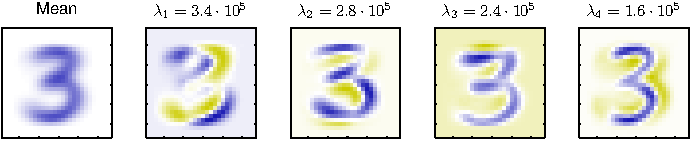
\includegraphics[scale=1.00]{./img/pca/handwritten_digit_eigenvectors}
		\caption{Anwendung der PCA auf einen Datensatz bestehend aus 6.000 Bildern mit $28 \times 28$ Pixeln. Positive Werte sind blau,
			negative Werte gelb dargestellt.
			Siehe \cite{Bishop2024}, Seite 502.}
	\end{figure}
\end{frame}


% Datenkompression (Forts.)
\begin{frame}{Datenkompression (Forts.)}{}
	\begin{figure}[H]
		\divideTwo{0.49}{
			\centering
			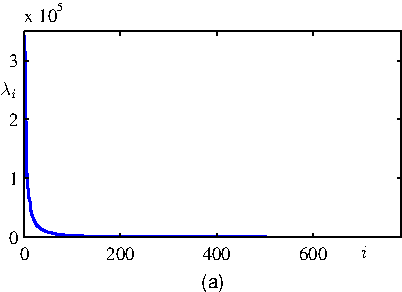
\includegraphics[scale=0.85]{./img/pca/handwritten_digit_eigenvalue_spectrum}			
		}{0.49}{
			\centering
			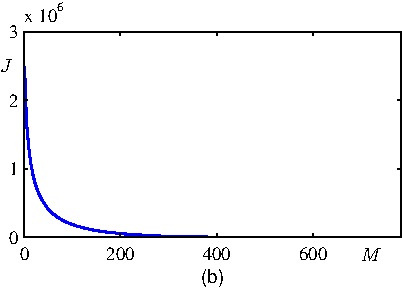
\includegraphics[scale=0.85]{./img/pca/handwritten_digit_error_measure}
		}
		\caption{(a) Plot des Spektrums der Eigenwerte in absteigender Sortierung. (b) Plot der Summe der verworfenen Eigenwerte (Fehler $J$).
			Siehe \cite{Bishop2024}, Seite 503.}
	\end{figure}
\end{frame}


% Datenkompression (Forts.)
\begin{frame}{Datenkompression (Forts.)}{}
	\begin{figure}
		\centering
		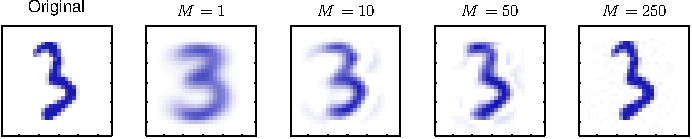
\includegraphics[scale=1.00]{./img/pca/handwritten_digit_reconstruction}
		\caption{Reduktion eines Elements des Datensatzes auf verschiedene Dimensionen. Bishop benutzt $M$ anstelle von $D$ für die Dimension
			des Unterraums. Siehe \cite{Bishop2024}, Seite 502.}
	\end{figure}
\end{frame}